\chapter{Power System Simulation Model Using MATLAB/Simulink}
\label{ch:chapter4}


\section{4.1  Introduction}
MATLAB/Simulink was selected as the primary simulation platform for this research due to its uniquely integrated environment that combines high-fidelity electromagnetic-transient modelling via Simscape Electrical with native machine-learning support through the Deep Learning Toolbox and ONNX runtime. This integration enables a seamless workflow from simulation-based data generation to DWT-LSTM model training, validation, and deployment within a single ecosystem. Simscape Electrical provides validated component models---saturable transformers, CTs with core saturation, circuit breakers, and programmable voltage sources---ensuring waveform-level fidelity essential for protection studies, and supports automated batch simulations via MATLAB scripting \cite{ref1, ref2}.

Figure 4.1: Overview of the MATLAB/Simulink power-system simulation model.


\section{4.2  MATLAB/Simulink Simulation Environment}

\subsection{4.2.1  Software Overview}
The simulation platform comprises MATLAB R2023a with Simulink, Simscape Electrical, the Deep Learning Toolbox, the Signal Processing Toolbox, and the ONNX converter for MATLAB. Simscape Electrical uses a physical-network approach where components enforce Kirchhoff's laws, with the underlying solver automatically constructing and solving network equations at each time step. The Deep Learning Toolbox supports import and inference of the trained DWT-LSTM model via ONNX \cite{ref3}.


\subsection{4.2.2  Solver Configuration}
A discrete-time solver with a fixed sample time of Δt = 1×10⁻⁵ s (10 µs) is employed, corresponding to a Nyquist frequency of f\_Nyquist = 1/(2Δt) = 50 kHz. This provides a 50× oversampling margin relative to the relay rate of 1600 Hz (32 samples/cycle at 50 Hz), ensuring negligible aliasing. The powergui block uses Discrete mode at 10 µs \cite{ref4}.


\subsection{4.2.3  Simulation Duration}
Each simulation runs for T\_sim = 1.0 s, with the event injected at t\_event = 0.2 s (10 cycles pre-event, 40 cycles post-event). At the relay sampling rate of 1600 Hz, N\_samples = 1600 × 1.0 = 1600; including the initial reference, each record contains 1601 samples (n = 0 to 1600), yielding 1601 - 32 + 1 = 1570 one-cycle sliding windows per case.


\section{4.3  Transformer Model Parameters}

\subsection{4.3.1  Transformer Rating and Configuration}
The protected transformer is a three-phase, 300 MVA, 230/11 kV unit with Yd1 vector group (grounded wye primary, delta secondary with -30° phase displacement), a prevalent configuration in transmission substations \cite{ref5}. The full-load currents are I\_FLA,HV = 300×10⁶/(√3·230×10³) = 753.1 A and I\_FLA,LV = 300×10⁶/(√3·11×10³) = 15 746 A. Per-unit base impedances are Z\_base,HV = 176.33 Ω and Z\_base,LV = 0.4033 Ω. Parameters are summarized in Table 4.1.

Table 4.1: Transformer Nameplate and Equivalent Circuit Parameters.


\subsection{4.3.2  Core Saturation Characteristics}
The Simscape Electrical saturable-transformer block models core nonlinearity through a piecewise-linear B-H curve specified as flux-linkage / magnetizing-current coordinate pairs, configured with 20 data points spanning ±2.0 p.u. flux and a knee point near 1.2 p.u. flux. Above the knee, incremental permeability drops to 0.2\% of the air-core inductance, reproducing the deep-saturation characteristic of grain-oriented silicon steel (M5 grade) \cite{ref6}. Worst-case inrush (α = 0°, φ\_r = +φ\_m) yields φ\_peak = 3φ\_m, producing inrush peaks of 5--10 times rated current \cite{ref7}.


\subsection{4.3.3  Three-Phase Winding Configuration}
The Yd1 group is implemented with the primary as ``Yg'' and secondary as ``D1'' (delta, -30° lag). The 30° displacement requires phase compensation before computing the differential current, performed by applying a -30° rotation to the LV-side CT currents via a Clarke transformation.


\section{4.4  Power System Network Model}

\subsection{4.4.1  Source Model and Equivalent Impedance}
The external system is represented by Thévenin equivalents on both sides \cite{ref8}. On the HV side (1.05 p.u. voltage, X/R = 30.0), Z\_th,HV = 0.5 + j15.0 Ω with a short-circuit level of 3 524 MVA. On the LV side (1.0 p.u. voltage), Z\_th,LV = 0.01 + j0.10 Ω with 1 204 MVA. Available fault currents are I\_f,HV = 8.84 kA and I\_f,LV = 63.2 kA, consistent with typical 230/11 kV substations.


\subsection{4.4.2  Breaker and Snubber Circuit}
Circuit breakers are modelled using the Simscape Electrical three-phase breaker block (R\_on = 0.001 Ω, R\_off = 10⁶ Ω). RC snubber circuits (R\_s = 1000 Ω, C\_s = 0.1 µF) are connected across each breaker to damp high-frequency switching transients and maintain numerical stability of the discrete solver \cite{ref9}.


\subsection{4.4.3  Load Model}
The LV-side load is a composite of 70\% constant impedance (168 MVA) and 30\% constant power (72 MVA), totalling 240 MVA at 0.85 lagging power factor (80\% transformer loading). A 2\% phase unbalance and a shunt capacitor bank for power-factor correction are included.


\subsection{4.4.4  Current Transformer Model}
CTs on both sides are modelled using the Simscape Electrical linear-transformer block with saturable core. Accurate CT modelling is critical since CT saturation during through-faults is a well-documented cause of differential-relay maloperation \cite{ref10}. CT saturation is modelled through a piecewise-linear flux-current curve. Parameters are given in Table 4.2.

Table 4.2: Current Transformer Parameters.


\section{4.5  Fault and Event Simulation Scenarios}

\subsection{4.5.1  Internal Fault Modeling}
Internal faults are simulated at five winding taps (5\%, 25\%, 50\%, 75\%, 95\%) using the three-phase fault block. Four fault types (SLG, LL, LLG, 3LG) are applied with three inception angles and three fault resistances (0.01 Ω, 5 Ω, 25 Ω). The effective fault impedance at tap p is Z\_fault(p) = p²Z\_k + R\_f. Terminal faults yield the highest currents; 720 deterministic cases are generated \cite{ref11}.


\subsection{4.5.2  External Fault Modeling}
External faults (SLG, LL, LLG, 3LG) are simulated on both HV and LV buses, representing faults outside the differential zone. Evolving faults (SLG → LLG after 3 cycles → 3LG after 6 cycles) are implemented via a Simulink state machine. Stress-test scenarios include asymmetrical CT saturation and fault currents ranging from 5 to 30 p.u., producing 540 deterministic external-fault cases \cite{ref12}.


\subsection{4.5.3  Inrush Current Simulation}
Inrush conditions are generated by sweeping the switching angle α across seven values (0° to 180° in 30° steps) and the residual flux φ\_r across nine values (-0.8 to +0.8 p.u.), yielding 63 combinations. Simulations include symmetric, asymmetric, and single-phase residual-flux distributions. Sympathetic inrush is modelled using two parallel transformers, producing 189 deterministic inrush base cases \cite{ref13}.


\subsection{4.5.4  CT Saturation Conditions}
CT saturation stress cases vary burden impedance (rated, 2×, 4×), fault-current magnitude (10, 20, 30× rated), and remanent flux (0, +0.5B\_r, +0.8B\_r), producing 108 dedicated cases spanning both bus sides and worst-case inception angles \cite{ref14}. These are grouped with external faults for classification (incl. CT saturation).


\subsection{4.5.5  Normal Operating Conditions}
Normal operating scenarios cover six load levels (0\% to 110\% rated), three tap positions, five voltage levels (0.95--1.05 p.u.), and three power factors. The steady-state differential current due to tap mismatch is I\_diff,tap = I\_load · Δ\_tap/(1 + Δ\_tap), yielding approximately 5\% of load current for a ±5\% tap change. A total of 270 deterministic normal-operating cases are generated \cite{ref15}.


\section{4.6  Automated Data Generation and Dataset Summary}
The batch simulation is automated via a MATLAB script (ControlPanel.m) that modifies Simulink parameters via set\_param, runs simulations in parallel using parsim, and post-processes results. The signal-conditioning pipeline emulates a merging unit: a 4th-order Butterworth anti-aliasing filter (800 Hz cut-off), 16-bit quantization, and AWGN at SNR levels of 20, 30, and 40 dB. After downsampling to 1600 Hz, each case yields a 1601-sample record per phase, exported to .mat files for the PyTorch training pipeline. Stochastic augmentation randomizes inception angle U(0°, 360°), fault resistance logU(0.01, 50) Ω, source impedance (±5\%), and fault location U(2\%, 98\%), expanding and balancing the deterministic base cases to a final dataset of 2,500 cases (3,200 per class) \cite{ref16}.

Table 4.3 presents the final augmented dataset of 2,500 cases, split into training (70\%), validation (15\%), and testing (15\%) subsets via stratified random splitting---yielding 8,960 training, 1,800 validation, and 1,800 testing cases. This corresponds to approximately 61.5 million sampled data points and 20.1 million one-cycle sliding windows for DWT-LSTM training.

Table 4.3: Final Augmented Dataset Summary.


\section{4.7  Signal Conditioning and Merging-Unit Emulation}
To ensure that the generated dataset reflects the measurement chain of a modern digital substation rather than idealised simulator output, each raw differential-current record is passed through a signal-conditioning pipeline that emulates an IEC 61850-9-2 merging unit. The pipeline comprises four stages applied in sequence: anti-alias filtering, decimation to the relay rate, quantisation, and noise injection. Table 4.4 lists the parameters of each stage.

Table 4.4: Merging-unit signal-conditioning pipeline parameters.

The 800 Hz anti-alias cut-off is matched to the 1.6 kHz Nyquist limit, attenuating components above the eighth harmonic that would otherwise alias into the DWT sub-bands. Sixteen-bit quantisation reproduces the dynamic range of contemporary analogue-to-digital front ends, introducing a quantisation floor well below the noise levels of interest. The additive white Gaussian noise model conservatively represents combined sensor, electromagnetic-interference, and transmission noise; the three nominal SNR levels populate the training set, while the 15 dB and 50 dB extremes are reserved for the out-of-distribution stress tests of Chapter 6. This conditioning chain is applied identically during data generation and during Simulink deployment, so that no distribution shift is introduced between training and inference.

Figure 4.2: Block diagram of the merging-unit signal-conditioning and noise-injection pipeline.


\section{4.8  Dataset Statistics and Class Balance}
The final balanced corpus comprises 3,200 cases per class (2,500 total), with stratified 70/15/15 partitioning preserving class proportions in every subset. Balancing is achieved by combining deterministic base scenarios (Section 4.5) with stochastic augmentation that randomises inception angle, fault resistance, source impedance, and fault location, ensuring that each class spans a comparable region of the operating-condition space. Figure 4.3 visualises the composition of the dataset across classes and subsets, and the parameter ranges spanned by the augmentation are summarised in Table 4.5.

Table 4.5: Stochastic augmentation parameter ranges.

Figure 4.3: Composition of the balanced 2,500-case dataset across classes and train/validation/test subsets.


\begin{figure}[htpb]
\centering
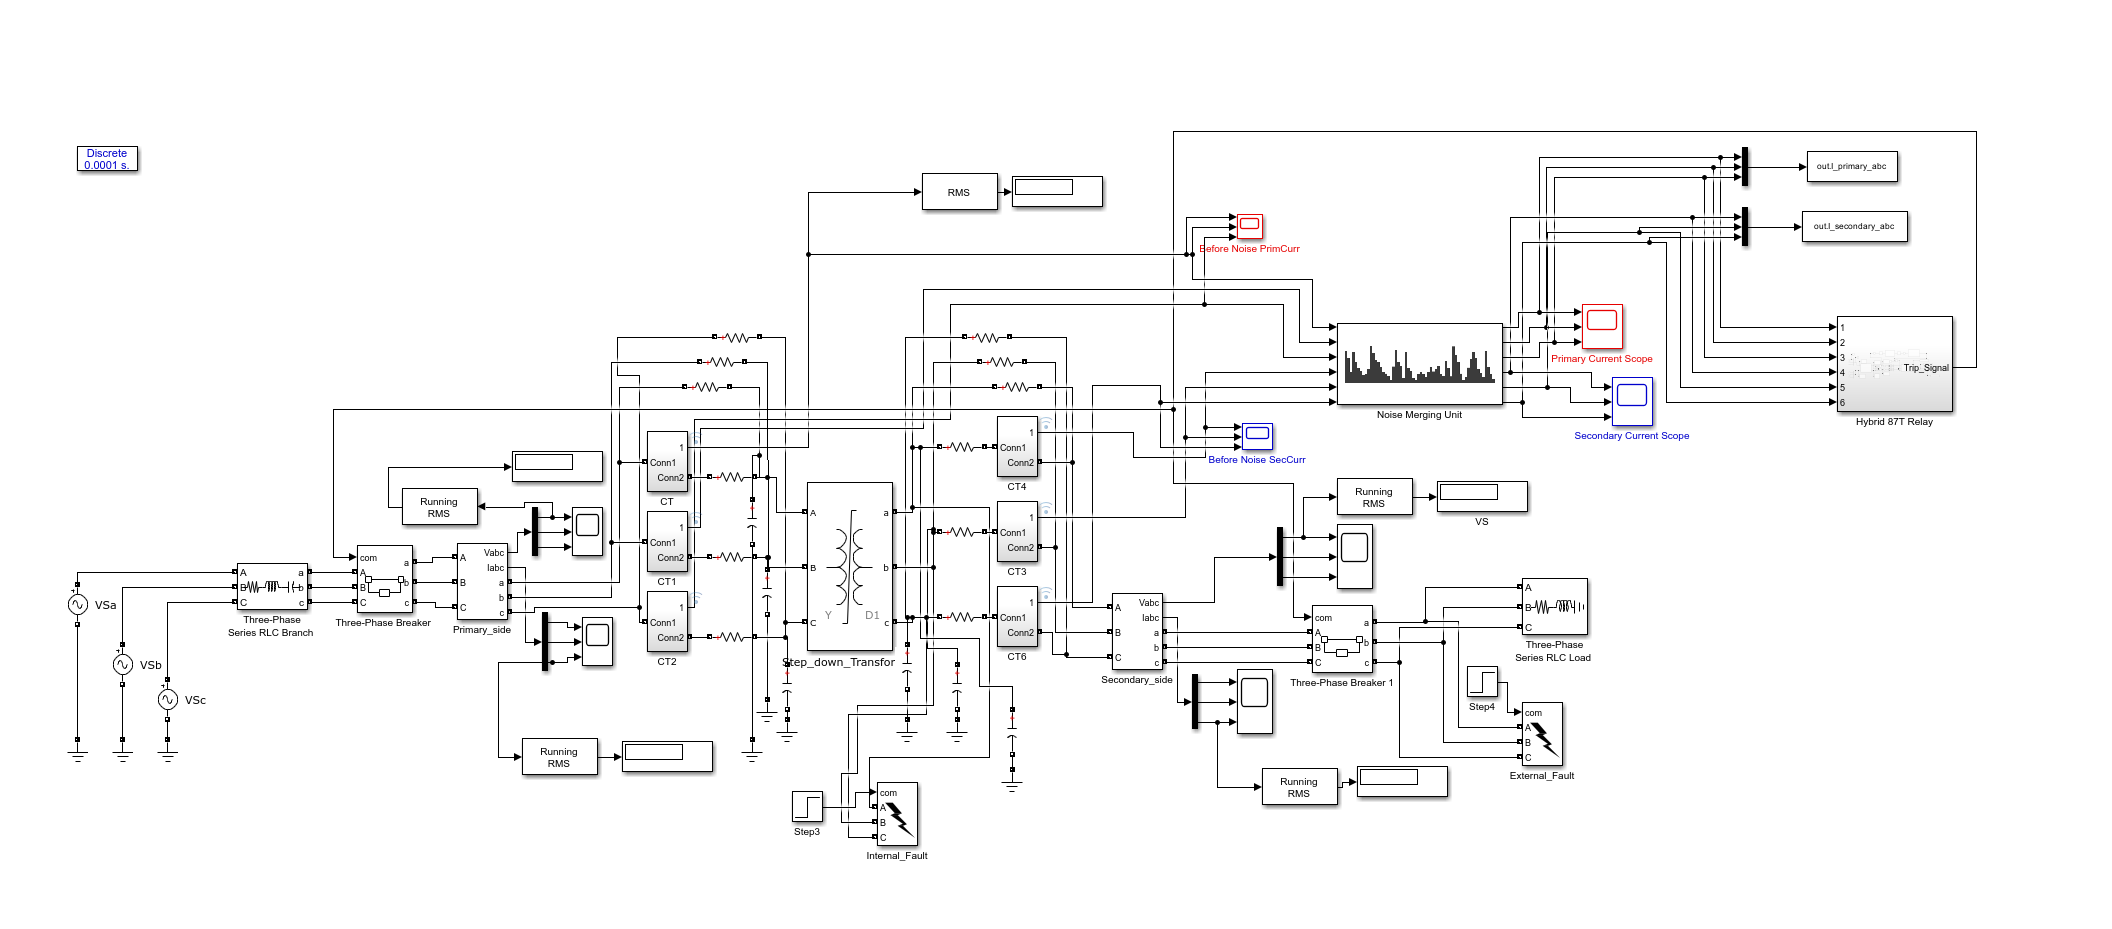
\includegraphics[width=0.75\textwidth]{figures/Main Panel.png}
\caption{Overview of the MATLAB/Simulink power-system simulation model.}
\label{fig:main_panel}
\end{figure}

\begin{figure}[htpb]
\centering
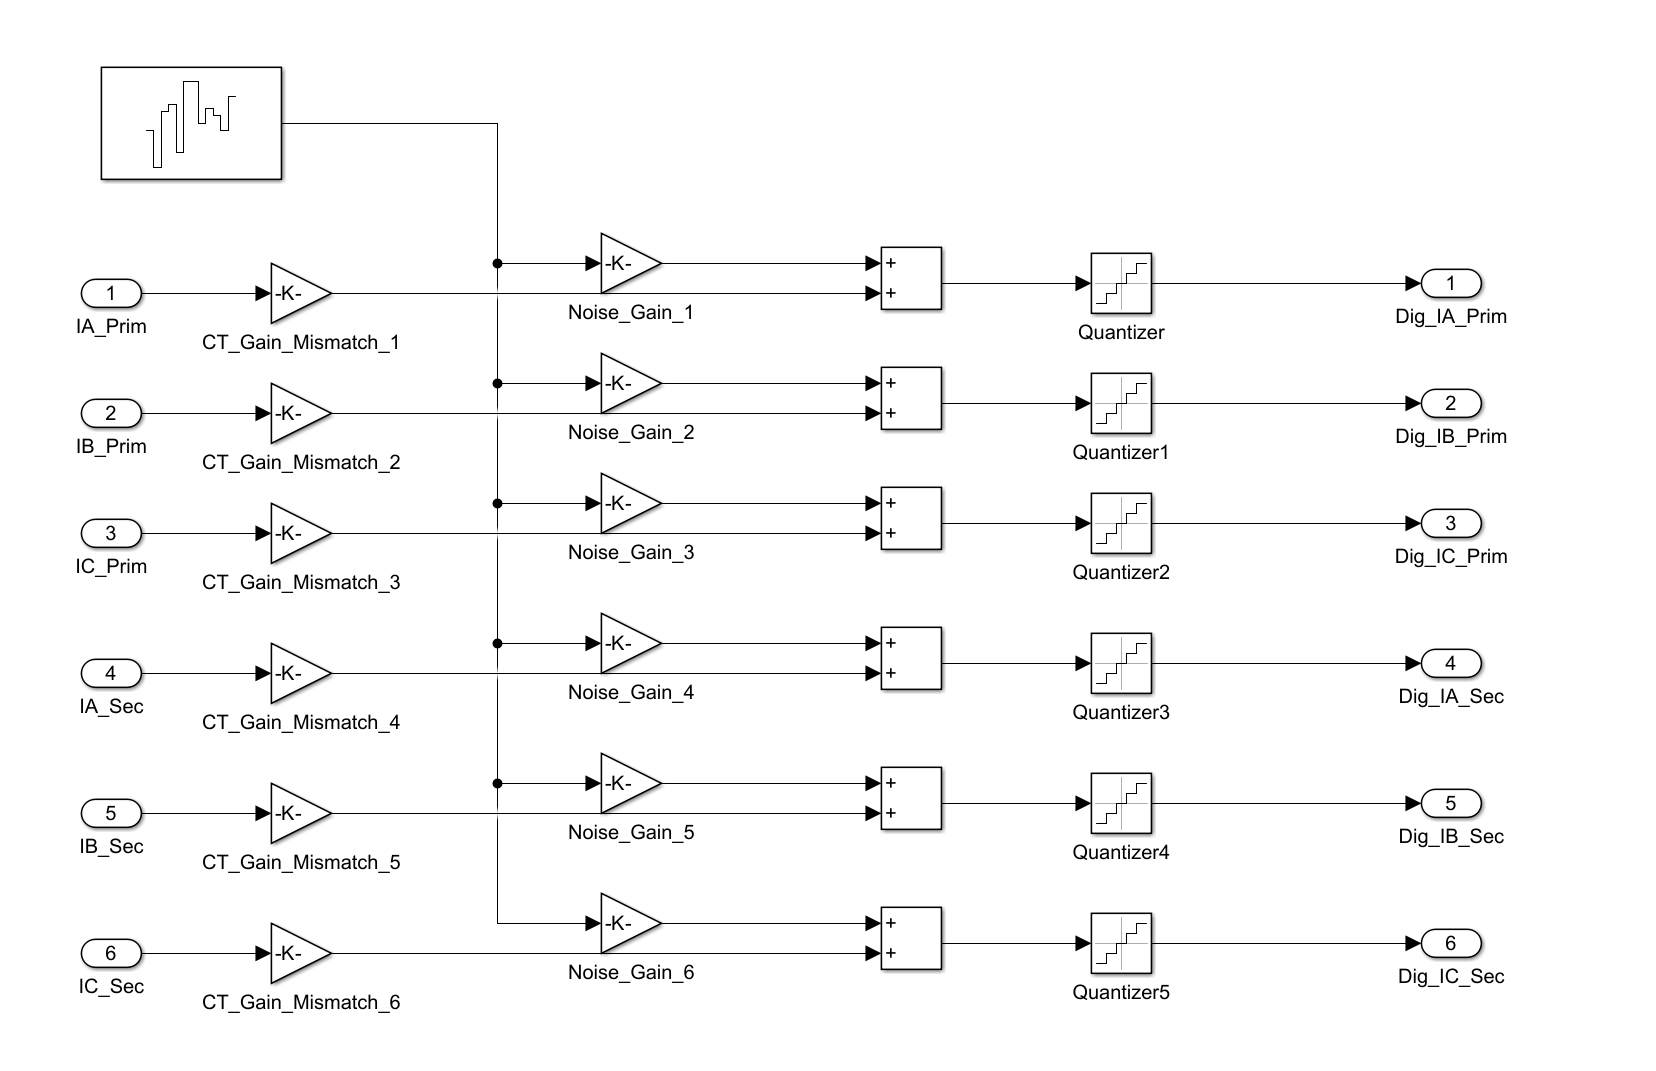
\includegraphics[width=0.75\textwidth]{figures/noise Merging Unit.png}
\caption{Block diagram of the merging-unit signal-conditioning and noise-injection pipeline.}
\label{fig:merging_unit}
\end{figure}

\begin{figure}[htpb]
\centering

\includegraphics[width=0.75\textwidth]{figures/academic_plots/12_Dataset_Composition.png}
\caption{Composition of the balanced 2,500-case dataset across classes and train/validation/test subsets.}
\label{fig:dataset_composition}
\end{figure}
